\documentclass[10pt]{article}

\usepackage[utf8]{inputenc}
\usepackage[portuges]{babel}
\usepackage{a4wide}
\usepackage{graphicx}
\usepackage[export]{adjustbox}
\usepackage[labelformat=empty]{caption}
\graphicspath{ {img/} }

\begin{document}

\title{Projeto de Laboratórios de Informática 3\\2ª Fase\\Grupo 34}
\author{Alexandre de Freitas Ferreira Pacheco A80760\and Diogo José Cruz Sobral A82523\and José Pedro Milhazes Carvalho Pinto A80741}


\date{\today}


\maketitle

\begin{figure}[h]
	\minipage{0.32\textwidth}\centering
		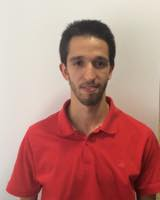
\includegraphics[scale=0.5]{A80760.png}
		\caption{A80760}
		\label{fig1:A80760}
	\endminipage\hfill
	\minipage{0.32\textwidth}\centering
		
\includegraphics[scale=0.5]{A82523.jpg}
		\caption{A82523}
		\label{fig2:A82523}
	\endminipage\hfill
	\minipage{0.32\textwidth}\centering
		
\includegraphics[scale=0.5]{A80741.jpeg}
		\caption{A80741}
		\label{fig3:A80741}
	\endminipage
\end{figure}


\begin{abstract}
		Como já foi visto, nesta unidade curricular foi-nos proposta 
	a implementação de um sistema de resposta a \textit{queries} 
	sobre um \textit{dump} da  base dados do site \emph{Stack 
	Overflow}.
		
		Era pretendido que esta segunda fase do projeto fosse
	desenvolvida em \emph{Java}. Pelo que o esperado era uma maior
	facilidade na implementação das soluções para qualquer problema 
	que surgisse e em atingir objetivos como o o encapsulamento das
	estruturas de dados e a abstração de código.
	
		Ao longo desta segunda fase do projeto não pudemos deixar 
	de notar a grande diferença, em termos de ferramentas disponíveis 
	e "comodidade", entre trabalhar em \emph{Java} e em \emph{C}.
\end{abstract}

\pagebreak

\section{Ferramentas Utilizadas} 

		À senelhança do que aconteceu na primeira fase do projeto,
	servimo-nos de uma biblioteca para efeturar o parsing dos 
	ficheiros \textit{xml}, que foi o \emph{Java SAXParser}.
	
		Por outro lado, para organizarmos as nossas estruturas de 
	dados, desta vez nem sequer considerámos implementar versões 
	nossas das estruturas, visto que o java já apresenta uma 
	API riquíssima em ferramentas para este propósito.
	
	
\section{Tipos e Estruturas de Dados}		

		De modo a conseguir responder às \textit{queries} propostas de forma eficiente, é natural
	que o mais importante é a forma como organizamos o grande volume de informação 
	presente nos \textit{dumps} disponibilizados.
		
		Primeiro, analisámos a informação contida em cada um dos ficheiros \textit{xml}
	disponibilizados por comunidade (e.g. \textit{android}, \textit{ubuntu}...) e o 
	que era pedido nas \textit{queries}, a fim de perceber quais os dados que seriam recorrentemente
	necessários.

	
\subsection{Tipos de Dados: \textit{Users} e \textit{Posts}}
	
		As entidades elementares na forma de descrever cada comunidade, 	à volta das quais
	gira a grande maioria da informação, são os \textit{users} e os 			\textit{posts}.
	
		Naturalmente, e semelhantemente ao que fizemos na 1ª fase, 
	para cada um destes objetos criámos uma classe, \texttt{MyUser} 
	e \texttt{MyPost}.
	
		Para representar as \textit{tags} bastou implementar uma 
	correspondência entre os seus nomes e \texttt{Ids}, como veremos 
	à frente.
	

\subsection{Organização dos Objetos de Posts e Users}
		Para organizar a informação utilizámos sobretudo a interface
	\emph{Map} do \textit{Java}.
	
		Organizámos os \textit{users} num \texttt{LinkedHashMap} em 
		que a chave são os \texttt{Ids}.
	
		Organizámos os \textit{posts}, tal como na primeira fase em
	duas estruturas separadas, para os poder procurar quer por data
	quer por \texttt{Id}.  Assim, ficaram num \texttt{LinkedHashMap} 
	semelhante ao dos \textit{users} e noutro \texttt{LinkedHashMap} 
	com as \texttt{LocalDate} como chave e uma lista de \textit{posts} 
	por cada data.
	
		Esta lista de \textit{posts} foi implementada numa classe 
	que definimos fazendo uso da interface \texttt{List} e um contador 
	de perguntas e respostas que é preenchido aquando do 
	\textit{loading.}
	
		A informação das \textit{tags} consiste num 
		\texttt{LinkedHashMap} cujas chaves são nomes das tags e 
		os valores são os \texttt{Ids} das mesmas.
		
	
\subsection{Outras Estruturas Auxiliares}
		
		Para além da organização essencial referida, decicidmos 
	implementar, ainda, estruturas auxiliares, que são úteis sobretudo 
	quando a resposta a determinadas \textit{queries} envolve calcular 
	um conjunto de perguntas mais respondidas ou um conjunto de 
	utilizadores com maior reputação.
	
		Estas estruturas consistem em dias listas, mais propriamente, 
	\texttt{ArrayList}. Um deles contém os \texttt{Ids} de todos os
	\textit{users} ordenados pelo número de posts que o respetivo
	\texttt{user} efetuou. O outro segue a mesma lógica, mas o 
	critério de ordenação é a reputação dos \textit{users}.
	
	
	
\pagebreak

\section{Modularização e Abstração de Dados}
		Como temos aprendido ao longo dos últimos tempos, são boas práticas as de 
	manter um código modular e abstraído do tipo de dados com que	trabalhamos.
	
	\subsection*{Encapsulamento}
	
		Em \textit{java} é bastante fácil de encapsular os dados, 
	uma vez que a própria linguagem já tem mecanismos que facilitam 
	esta prática, como a simples declaração de variáveis de instância 
	como \texttt{private}. A fim de impossiblitar a propagação de 
	apontadores da estrutura interna da nossa comunidade, todos os
	\textit{sets} e \textit{gets} das classes que criámos trabalham 
	com clones. Os sets clonam a informação que recebem, e os gets 
	clonam a informação interna para devolver o clone.
	
	
	
	
	\subsection*{}
		A utilização das APIs do \textit{Java} tornou o código 
	bastante abstrato, visto que a qualquer momento podemos mudar, 
	por exemplo, o nosso programa para implementar os mapas num 
	\texttt{TreeMap} em vez de \texttt{LinkedHashMap} e pouco ou 
	nada termos de mudar. Este comportamento verifica-se na maior 
	parte do código.

\section{\textit{Queries}}
		Nesta secção passamos a explicar a abordagem que tomámos 
	em relação a cada uma das \textit{queries}, note-se que muitas 
	delas funcionam como na primeira fase.
	\subsection*{\textit{Query} 1 - Título e autor da pergunta}
		O procedimento que tomamos é bastante simples. 
		\begin{enumerate}
		\item Procuramos o post com o \texttt{Id} fornecido e verificamos se se trata
		 de uma pergunta. 
		\begin{enumerate}
		\item Se for uma pergunta, devolvemos o seu título e o \texttt{DisplayName} do autor 
	(procurado o \texttt{OwnerUserId} na árvore de users).
	
		\item Se for uma resposta, repetimos o ponto \textbf{1} com o \texttt{ParentId}
		do post, que será o \texttt{Id} da pergunta correspondente.
		\end{enumerate}
		\end{enumerate}
	\subsection*{\textit{Query} 2 - Top N \textit{users} com mais posts}
			Esta query toma partido da estrutura auziliar em que,
		aquando do \textit{load}, ordenamos os users pelo seu 
		número de \textit{posts}. Copia-se desta estrutura os 
		N primeiros utilizadores (ou todos, caso N seja maior
		que o tamanho desta coleção).			
	\subsection*{\textit{Query} 3 - Número de perguntas e respostas ao longo de um período}
			Como já referido, a árvore que organiza os \textit{posts} por data, em cada nodo,
		tem um array de posts. Para além do array propriamente dito, com apontadores do tipo
		\texttt{MYPOST}, há dois contadores: um para o número de respostas, e outro para o
		número de perguntas nesse array (calculados no \texttt{load}). Ora, é desta organização
		que esta \textit{query} toma partido.
		\begin{enumerate}
			\item Percorre-se os nodos da árvore de posts dentro do período especificado.
			
				Em cada nodo da árvore, soma-se os respetivos contadores à variável cujo 
			endereço é passado como argumento pela função de travessia.
		\end{enumerate}
	\subsection*{\textit{Query} 4 - Perguntas com determinada \textit{tag} feitas num período}
		\begin{enumerate}
			\item Percorre-se todos os nodos da árvore de posts dentro do período especificado.

				Percorre-se o \textit{array} de posts em cada nodo, e em cada post verifica-se
			se este é uma pergunta e contém a tag especificada. Se for esse o caso, adiciona-se
			o \texttt{Id} a um \textit{array} resultado (de onde posterioremente se passarão
			os valores para \texttt{LONG\_list})

		\end{enumerate}
			
	\subsection*{\textit{Query} 5 - Informação de um \textit{user} e os seus últimos \textit{posts}}
			Esta \textit{query} consiste em simplesmente procurar um utilizador na nossa estrutura
		e devolver a sua informação.			
			O tipo de dados \texttt{MYUSER} contém, como já foi visto, um \textit{array} com
		os \texttt{Ids} dos seus posts,o que facilita imenso esta resposta.
	\subsection*{\textit{Query} 6 - N respostas mais votadas ao longo de um período}
			A diferença entre os \textit{upvotes} e \textit{downvotes} de uma resposta
		equivale ao seu parâmetro \texttt{Score}, pelo que este já se encontra calculado
		a partir do momento em que o carregámos do ficheiro \textit{xml}.
			\begin{enumerate}
				\item São visitados todos os nodos da árvore de \textit{posts} dentro
					do período especificado, percorrendo o \textit{array} de \textit{posts}
					em cada nodo e inserindo numa \texttt{HEAP} (\textit{max-heap}) o par de
					informação \{\texttt{Id}, \texttt{Score}\}.
				\item Dá-se \textit{pop} a N elementos da heap e preenche-se a lista 
					resultado com os \texttt{Ids} das respostas a ser retiradas da \textit{heap}.
			\end{enumerate}
	\subsection*{\textit{Query} 7 - N perguntas com mais respostas ao longo de um período}
			Dado que as respostas às perguntas a devolver têm de ter sido feitas ao longo
		do período especificado, esta \textit{query} não se resume a consultar o número
		de respostas em cada pergunta no período de tempo, mas a calcular o número de 
		respostas feitas ao longo desse período para cada pergunta.
			\begin{enumerate}
				\item Percorre-se todos os \textit{posts} criados no período de tempo
					dado.
					\begin{enumerate}
						\item Percorre-se a lista de filhos desse \textit{post} (que só
							existe se este for uma pergunta) e conta-se quantos foram
							criados no período de tempo especificado.
						\item Insere-se numa \texttt{HEAP} (\textit{max-heap}) o par de  
							informação \{\texttt{Id}, número de respostas\}.
					\end{enumerate}
				\item Faz-se \textit{pop} a N elementos da \textit{heap}, guardando 
					na lista resultado os \texttt{Ids} das perguntas nas condições
					especificadas.
			\end{enumerate}
	\subsection*{\textit{Query} 8 - N perguntas mais recentes com determinada \textit{tag}}
			A query 8 não exige que todos os \textit{posts} sejam consultados,
		uma vez que estes se encontram organizados por tempo, e assim, podemos obter tudo o que 				precisamos visitando o número	mínimo de posts.
		
			O critério que utilizámos para determinar se a palavra ocorre ou não em cada
		título (para além de obviamente essa sequencia de caracteres aparecer na \textit{string}
		do título) foi a existência de espaços, pontuação, \textit{newline} ou \texttt{EOF}
		nas extremidades da \textit{substring} com a palavra. Para nos facilitar este trabalho
		utilizámos as funções de biblioteca \texttt{ispunct()} e \texttt{isspace()}.
			\begin{enumerate}
				\item Efetua-se uma travessia semelhante à \textit{inorder} na ordem
					"posts recentes - posts antigos". Que termina quando todos os
					nodos da árvore tiverem sido percorridos ou quando obtivermos N
					\textit{posts} nas condições pretendidas.
					\begin{enumerate}
						\item	Em cada nodo, percorre-se o array de \texttt{MYPOST}, e em cada 
						\textit{post} verifica-se se este contém a \textit{tag} especificada.
						Sendo esse o caso, adiciona-se o \texttt{Id} do \textit{post} a um
						\textit{array} (que posteriormente é passado para a \texttt{LONG\_list} 
						resultado).
					\end{enumerate}
			\end{enumerate}
	\subsection*{\textit{Query} 9 - N perguntas mais recentes em que dois \textit{users} participaram}
			Esta é outra query em que se tira bastante partido do facto de termos, no \texttt{load},
		carregado para o tipo \texttt{MYUSER} um array \texttt{STACKPOST} com os posts de cada
		\textit{user}.
			\begin{enumerate}
				\item São procurados os dois \textit{users} a partir dos \texttt{Ids} especificados e verifica-se qual dos dois tem menos posts.
				\item São percorridos os \textit{posts} desse user e são inseridos numa tabela
de \textit{hash} os \texttt{Ids} das perguntas relativas a cada post (ou seja, o próprio
\texttt{Id} se o \textit{post} for uma pergunta, ou o \texttt{ParentId} se o mesmo for uma
resposta).
				\item É repetido o processo para o outro utilizador, mas em vez de se inserir
na tabela \textit{hash} os \texttt{Ids}, verifica-se se estes estão já inseridos na tabela.
Aqueles que já estiverem são constituintes do reultado, sendo armazenados num \textit{array}
\texttt{STACKPOST}.
				\item Os elementos deste \textit{array} são ordenados segundo um algoritmo
\textit{quicksort} (segunda a sua \texttt{CreationDate}, e os N mais recentes são passados
para a \texttt{LONG\_list} resultado.
			\end{enumerate}
	\subsection*{\textit{Query} 10 - Melhor resposta}
			Esta \textit{query} é relativamente simples, devido ao facto de no \texttt{load} 
			armazenarmos um \textit{array} \texttt{STACKPOST} que guarda as respostas a cada 
			pergunta.
			\begin{enumerate}
				\item É procurada a pergunta na árvore ordenada por \texttt{Ids}.
				\item É percorrido o \texttt{STACKPOST} das respostas à pergunta e para cada
					um deles é calculada a pontuação (segundo a fórmula especificada no enunciado)
					e registado a melhor pontuação bem como a respetiva resposta, cujo \texttt{Id}
					é depois retornado. 
			\end{enumerate}
	\subsection*{\textit{Query} 11 - N \textit{tags} mais usadas ao longo de um período pelos N \textit{users} com maior reputação}
			Esta \textit{query} faz uso de grande parte das estruturas que temos montadas, bem
		como de estruturas criadas ao longo da sua execução.
		
			Nesta query, é criada uma tabela de \textit{hash} com as ocorrências de cada
		\textit{tag}. É ainda criada uma \texttt{HEAP} (\textit{max-heap}) onde depois são inseridos
		os \texttt{Ids} das \textit{tags} e as suas ocorrências como chave, de modo a ficarem 
		ordenados.
			É ainda importante mencionar que, na nossa interpretação do que foi pedido,
		utilizámos os N utilizadores com maior reputação de sempre (mesmo que não tenham
		postado nesse período de tempo). No resultado da query, \texttt{Ids} de tags com
		o mesmo número de ocorrências estão em ordem crescente.		
		
			\begin{enumerate}
				\item É obtido um array com os \texttt{Ids} dos N \textit{users} com
					maior reputação (procedendo da mesma forma que na \textit{query} 2, mas em
					relação à reputação e não ao número de posts).
				\item O array obtido é percorrido, procurando cada \texttt{Id} na árvore dos
					\textit{users} e obtendo  o \texttt{STACKPOST} com os \textit{posts}
					criados por cada um desses utilizadores.
					\begin{enumerate}
						\item Se o \textit{post} for uma pergunta e tiver sido criado dentro
							do intervalo de tempo especificado;
						\item Percorre-se cada \textit{tag} desse \textit{post} e, consultando 
						 a tabela de \textit{hash} pré-calculada, obtém-se o \texttt{Id} da mesma.
						\item Se este \texttt{Id} já constar na outra tabela de \textit{hash} que
							faz corresponder cada \texttt{Id} ao seu número de ocorrências, é 
							incrementado esse número. Caso contrário, esse \texttt{Id} é inserido.
					\end{enumerate}
				\item Preenchida a tabela \textit{hash} que a cada \texttt{Id} faz corresponder
				o seu número de ocorrrências, percorre-se todas as entradas da mesma e insere-se
				o par \{número de ocorrências, \texttt{Id}\} numa \textit{max-heap}, ficando assim
				os \texttt{Ids} ordenados.
				\item É feito \textit{pop} de N elementos da \texttt{HEAP}, e preenche-se a
				\texttt{LONG\_list} resultado com os \texttt{Ids} desses elementos.
			\end{enumerate}
\pagebreak

\section{Estratégias para melhorar a Eficiência}
		Tendo em conta o grande volume de dados que nos propusemos a processar neste projeto,
	surge a necessidade de adotarmos estratégias que melhorem a eficiência das operações que
	levamos a cabo.
	
			Uma decisão que tomámos de modo a melhorar a eficiência
	foi qual implementação da interface \texttt{Map} utilizar.
	Utilizámos \texttt{LinkedHashMap} porque, uma vez que é 
	implementada utilizando listas ligadas, nunca tem espaços vazios 
	que precisem de ser atravessados numa travessia (efetuada 
	em qualquer procura por um valor, se recordarmos o funcionamento 
	de uma tabela de \textit{hash}). 
	
		A única pequena desvantagem dos
	\texttt{LinkedHashMap} em relação aos \texttt{HashMap} é na 
	criação e inserção de valores, no entanto, foi um compromisso que 
	estivemos dispostos a fazer, dado que estas estruturas são criadas 
	durante o \textit{load}.
	
		Outra forma de tornar o nosso programa mais eficiente foi, 
	durante o \texttt{load}, construir estruturas auxiliares que, 
	embora armazenassem informação que pudesse ser obtida a partir 
	das árvores de \textit{posts} e \textit{users}, e levassem a um 
	ligeiramente maior gasto de memória, eram úteis a muitas 
	\textit{queries} e poupavam imensos cálculos e travessias.
	
	
		Uma prática que procurámos ter foi a utilização de arrays 
	sempre que possível. Um bom exemplo da nossa "aproximação" aos 
	\textit{arrays} é o facto de utilizarmos \texttt{ArrayList} nas 
	estruturas que nos devolvem os N \texttt{users} com mais reputação 
	ou \texttt{posts} efetuados.
	


\section{Conclusão}
	Tal como na primeira fase pudemos concluir, há sempre um 
compromisso performance vs. segururança, a organização da nossas 
estruturas toma um papel central nos fatores que influenciam a 
eficiência das \textit{queries}.
	
		
	Verificámos o esperado, que era ser muito mais simples implementar 
esta solução em \textit{Java} do que em C, dado o leque de ferramentas 
(a maior parte nativa da linguagem) com que pudemos contar para 
resolver qualquer problema.

	Resta refletir sobre as duas fases do projeto e afirmar que 
muito dificilmente, se nos propusessem novamente uma tarefa 
semelhante, escolheríamos C para implementar a solução. No fundo, 
apenas uma ínfima parte dos projetos requerem virtudes que apenas 
linguagens como o C podem oferecer. Num mundo cada vez mais 
orientado aos objetos e exigente por por produtividade, é natural 
que vigore a utilização de linguagens com um maior nível de abstração.

\end{document}\grid
\grid\grid
\grid
